\documentclass{article}
\usepackage[utf8]{inputenc}
\usepackage{graphicx}
\usepackage{amsthm}
\usepackage{amssymb}
\usepackage{amsfonts}
\usepackage{color}
 \usepackage{wrapfig}

\title{TP3\\ Equations différentielles}
\author{BRAHMI Kahina et HARDY Marion}

\begin{document}
\maketitle

	Ce TP,illustre plusieurs méthodes pour intégrer numériquement sur un intervalle une équation différentielle ordinaire.

\section{EXERCICE : EDO : $u'(t)=-u(t)$}

Nous avons tout d'abord identifié ce que vaut la fonction $f$ (respectivement $u(t)$). Pour cet exemple, nous avons pris la fonction exponentielle suivante: $e^-^t$. Nous avons calculé et dessiné la solution $u$ de l'EDO ci-dessus sur l'intervalle [0,2] ($cf.annexe$).

\begin{center}
	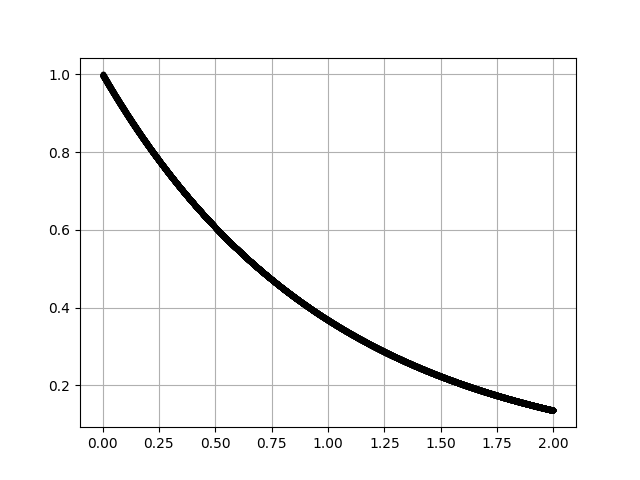
\includegraphics[scale=0.5]{graph2.png}
\end{center}

\newpage

\section{EXERCICE : méthode d'Euler}

Nous avons calculé une suite d'approximations $u_{k}$ où $u_{k+1}$ = $u_{k}$ + $hf(t_{k},u_{k})$ en posant $u_{0}$=1.0. Autrement dit nous avons calculé les $n$+1 premiers termes de la suite ($u_{k}$) en posant $T$ = 2.0 et $n$ = 10. 

\begin{center}
\begin{tabular}{| r | r |}
\hline
{premier terme} & $0.8$\\
\hline
{deuxieme terme} & $0.64$\\
\hline
{troisieme terme} & $0.512$\\
\hline
{quatrieme terme} & $0.4096$\\
\hline
{cinquieme terme} & $0.32768$\\
\hline
{sixieme terme} & $0.262144$\\
\hline
{septieme terme} & $0.2097152$\\
\hline
{huitieme terme} & $0.16777216$\\
\hline
{neuvieme terme} & $0.134217728$\\
\hline
{dixieme terme} & $0.1073741824$\\
\hline
\end{tabular}
\end{center}

Représentés par le graphique ci-dessous : 

\begin{center}
	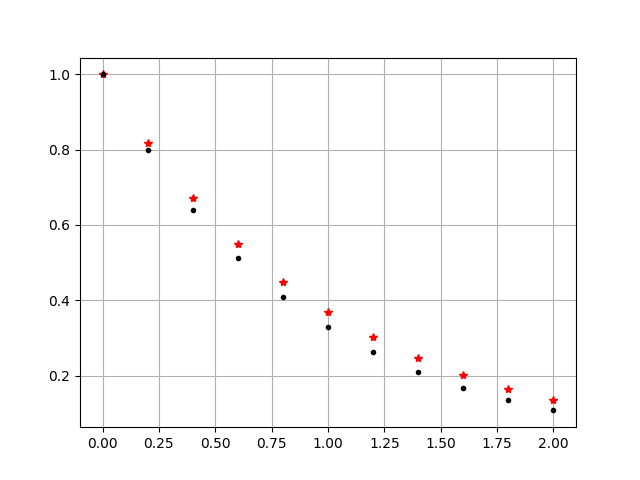
\includegraphics[scale=0.5]{CourbeU.png}
\end{center}

Puis nous avons représenté sur le grapique qui suit, 

\begin{center}
	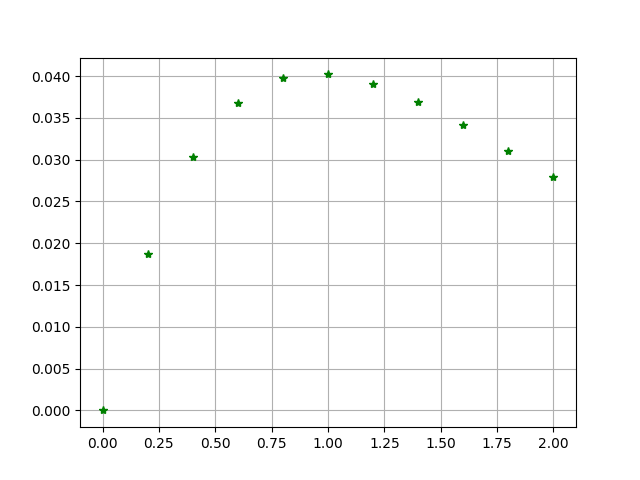
\includegraphics[scale=0.5]{erreur_exo2.png}
\end{center}

\section{EXERCICE : Fonction Euler}

Nous avons définie une fonction {\bf euler} en python qui prend en argument quatre variables, la fonction f ci-dessus, un $u_{0}$, un réel $T$ représentant la borne supérieure de l'intervalle et un entier $n$ servant à diviser l'intervalle en parties égales ($n$ se trouvant le nombre de parties égales). En appliquant la fonction euler à l'exercice précédent on a pu retrouver les résultats obtenus auparavant.

\section{EXERCICE : Fontion Euler 2}

En effet, nous avons défini la fonction $F$ tel que $U'(t)=F(t,U(t))$. Puis nous avons modifié la fonction {\bf euler} pour qu'elle prenne en argument une fonction $F$ qui elle même prend en argument un flottant $t$ et un numpy array de taille 2 $U$, la fonction {\bf euler} prend également une valeur initiale $U_{0}$, un flottant $T$ et un entier $n$. La fonction {\bf euler} modifié renverra tout comme auparavant deux \textbf{ numpy arrays} mais les tailles diffères des tailles des \textbf{ numpy arrays} de la première fonction {\bf euler}. Enfin on a resolu l'equation différentielle ordinaire en prenant $w$=1.0, $T$=4pi et en posant $u(0)$=1.0 et $u'(0)$=0.0.

\begin{center}
	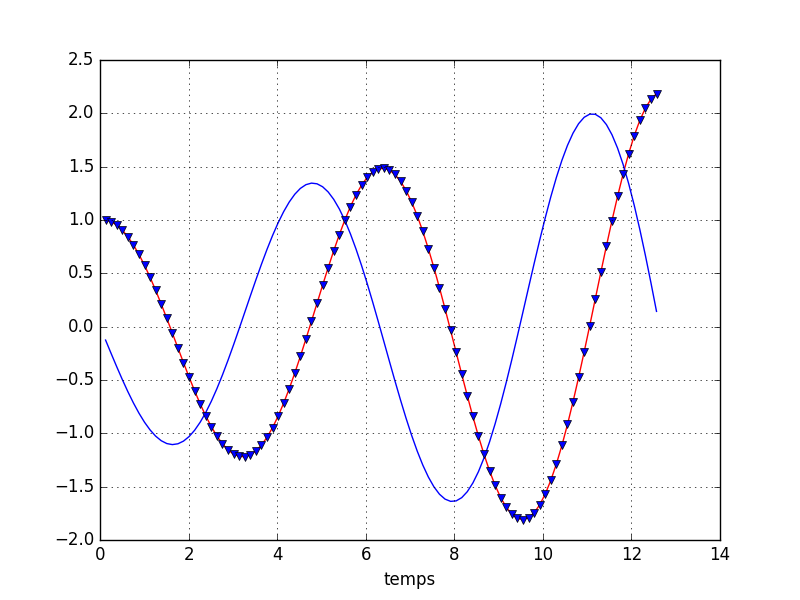
\includegraphics[scale=0.5]{graphe4.png}
\end{center}

\end{document}

